\documentclass[english,10pt,a4paper]{article}
\usepackage[utf8]{inputenc}
\usepackage[T1]{fontenc}
\usepackage{float}
\usepackage{babel}
\usepackage{amssymb}
\usepackage{graphicx}
\usepackage{hyperref}
\usepackage{mathtools}
\usepackage{amsthm}
\usepackage{nameref}
\usepackage{thmtools}
\usepackage{xcolor}
\usepackage{tikz}
\usepackage[european resistors]{circuitikz}
\hypersetup{
	pdfborder = false,
	colorlinks=true,
	linkcolor=black,
	filecolor=black,      
	urlcolor=blue,
	pdftitle={Overleaf Example},
	pdfpagemode=FullScreen,
}
\title{Stylophone\\
	\normalsize 555 timer}
\author{Kamil Chaj}
\date{2023}

\begin{document}
	\maketitle
	\tableofcontents
	\newpage
	
	\section{Introduction}
	
	\subsection{Stylophone}
	Stylophone is pocket synthesizer which uses voltage-controlled oscilator controlled with stylus which closes circuit in different position on metal keyboard on printed circuit board.
	\begin{figure}[H]
		\centering
		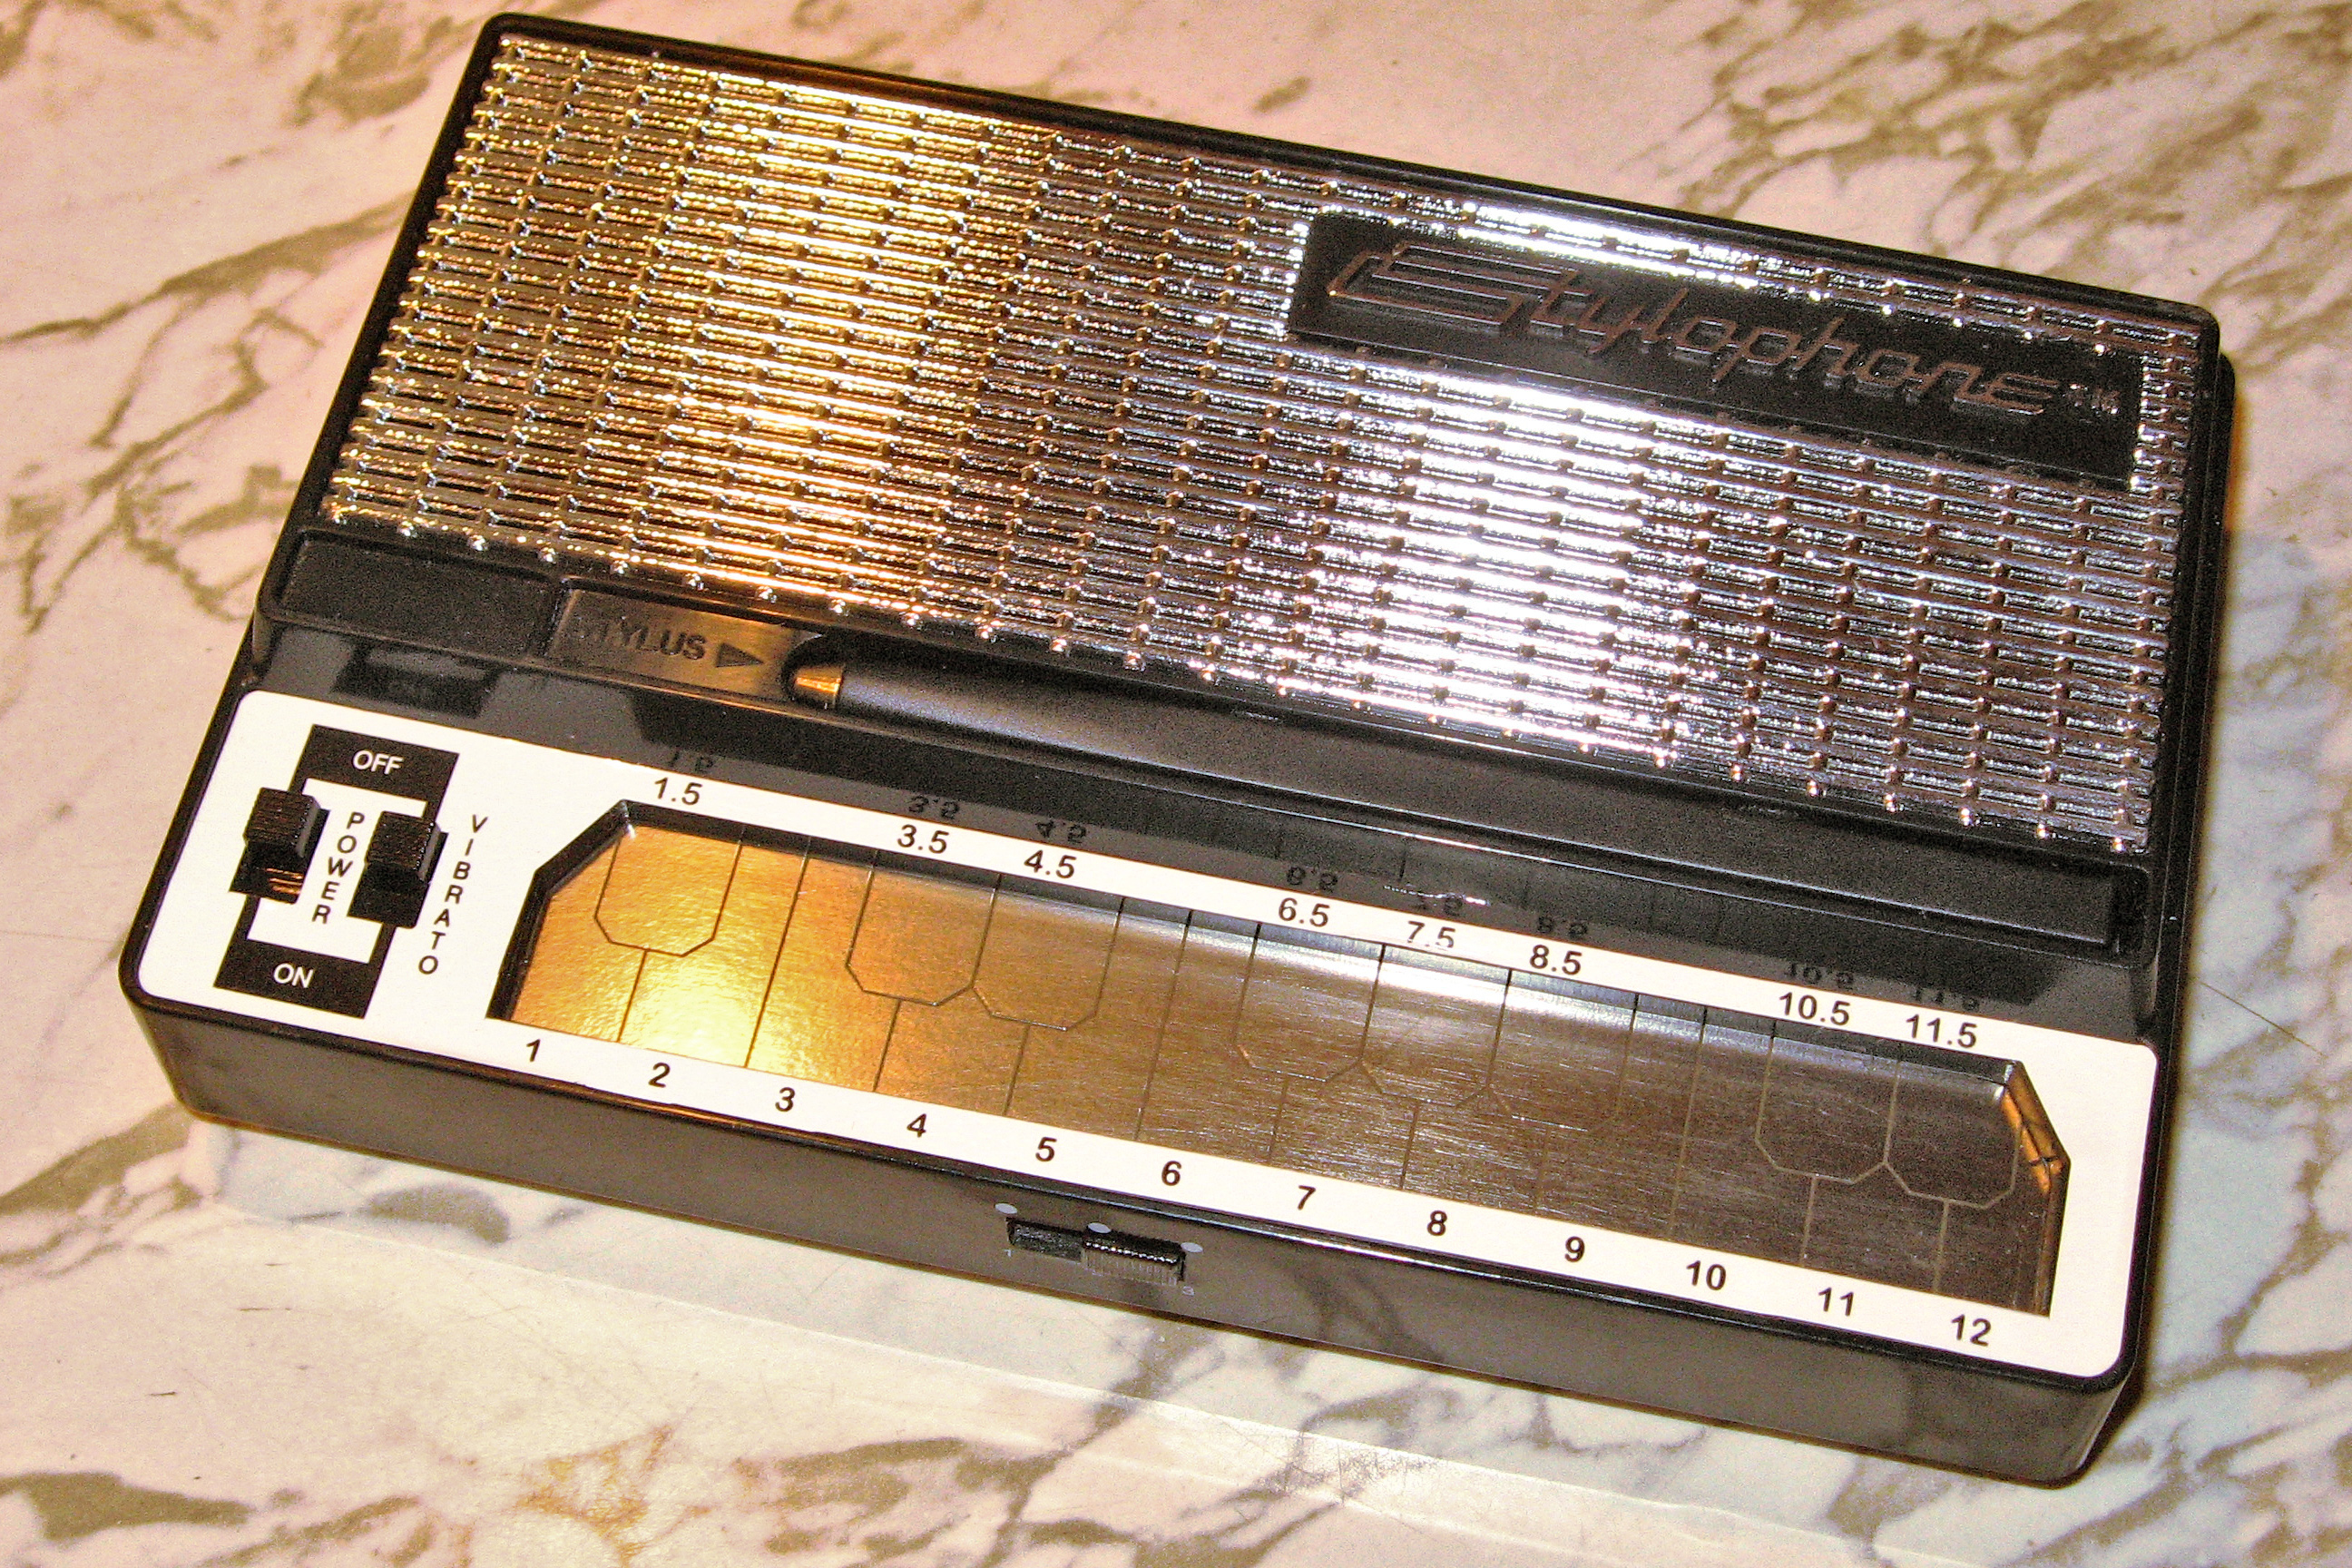
\includegraphics[width=0.6\textwidth]{img/Modern_Stylophone.jpg}
		\caption{Stylophone 2007}
	\end{figure}
	
	\subsection{Goal}
	Voltage controlled oscillator compatible with octave per volt standard, generation of saw tooth and square wave, vibrato effect and supplied with single pole supply.	
	
	\subsection{History}
	Stylophone was invented by Brian Jarvis of Dubreq Studios in 1967 and initialy was produced from 1968 to 1975, but in 2007 production of stylophone was relunched. Version of stylophone from 2007 used digital electronics unlike original but in 2020 Dubreq released new analog version of stylophone which uses 555 timer integrated circuit as its heart.
	
	Number of widly known artists used stylophone in the past like The White Stripes, David Bowie or Jarvis Cocker. These days stylophone can be heard in various genres or in full stylophone covers of popular songs.
	
	\subsection{555 integrated circuit}
	555 integrated circuit, designed in 1971 by Hans Camenzind, is said to be the most popular integrated circuit ever made. 555 can be used in many configuration like: oscilators, schmit triggers, SR latches and many more.
	
	\begin{figure}[H]
		\centering
		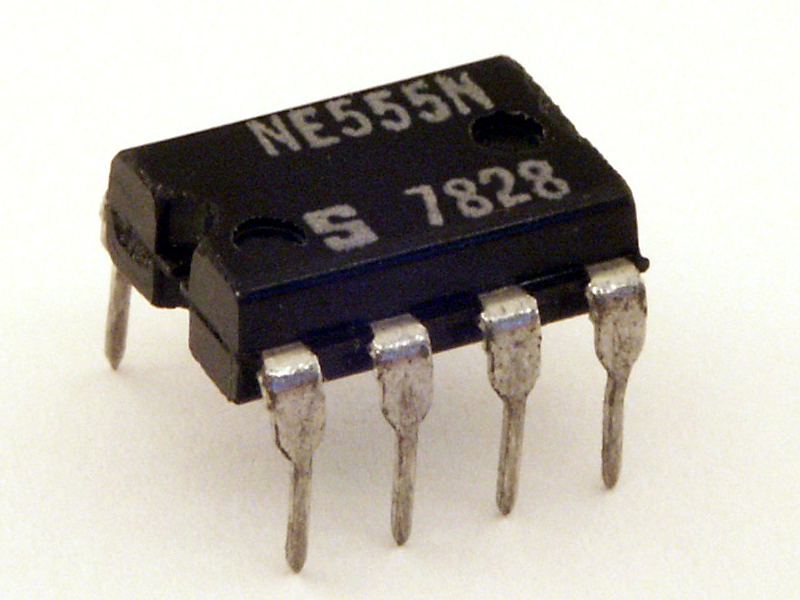
\includegraphics[width=0.6\textwidth]{img/Signetics_NE555N.JPG}
		\caption{Signetics NE555N}
	\end{figure}
		
	Output of 555 IC can be either high or low it is dependent on state of flip-flop which is controller with 2 comparators, when voltage on pin 2(trigger) is smaller than 1/3 of supply voltage comparator sets flip-flip and output is high and stays that way until flip-flop is reset by pin 4(reset) or when voltage on pin 6(threshold) is greater than 2/3 of supply voltage.
		
	\begin{figure}[H]
		\centering
		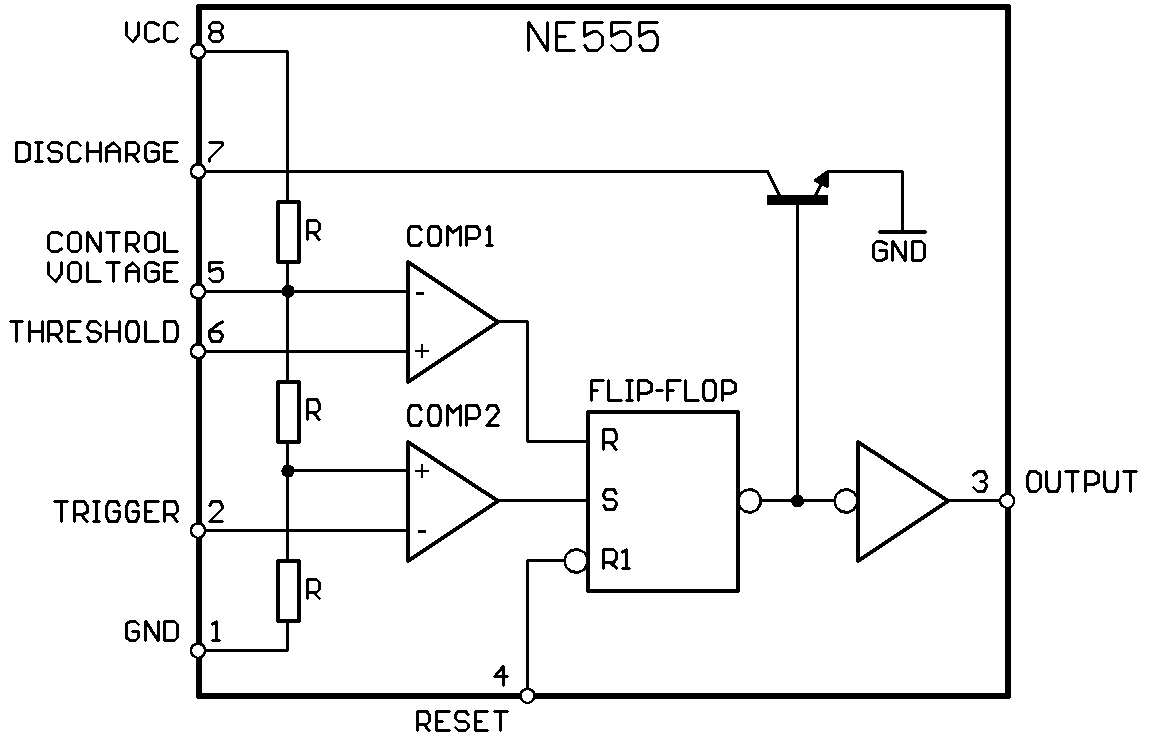
\includegraphics[width=0.6\textwidth]{img/555_esquema.png}
		\caption{Signetics NE555 internal block diagram}
	\end{figure}
	
	\section{Design}
	\subsection{VCO}
	In our circuit we are going to utilize similar idea to example oscillator circuit from documentation of 555 IC. When voltage over capacitor is greater than $\frac{2}{3}$ of supply voltage output is high and when it falls below $\frac{1}{3}$ of supply voltage output is low.
	
	This way we can generate many different waveforms like sawtooth or square depending on speed of charging and discharing of the capacitor.
	
	In example circuit from documentation resistance was used to control charging and discharging of capacitor which doesn't satisfies us, we want to use voltage therefor instead of resistors we are going to used bipolar junction transistors.
	\subsubsection{Capacitor}
	
	\begin{equation}
		i = C \dfrac{dV_c}{dt}
	\end{equation}
	
		

	
	
	
\end{document}